%!TEX root = ../thesis.tex
\chapter{Introduction}  % Main chapter title
\label{cha:introduction}

\section{Towards the characterization of Exoplanets}

The field of exoplanetary science is rapidly accelerating with huge scientific and instrumental investment with the ultimate goal of detecting and characterizing a Earth-like planet, with the potential for life (as we know it). Since the very first exoplanet detection~\citet{ mayor_jupitermass_1995} the number of confirmed \footnote{Validated by more than one detection method} exoplanets has ballooned to over 3790 with almost another 3000 candidates awaiting confirmation\footnote{as of October 2018}. However, simply detecting the presence of exoplanets is not nearly enough to satisfy our quest for knowledge. There is an exorbitant amount to be gained through the full characterization of these known exoplanets.

When an Earth-twin planet is suspected (there have been several false claims already \textbf{e.g. mullally et al 2018)\citet{mullally_keplers_2018} other earth like planets shown tonot be earth like. papers} a full characterization is required confirm it's habitability \textbf{(ref)}. For instance, knowing only the mass and radius can provide an average density but not the composition or the internal structural make up~\citet{a paper about composition degeneracy}. The presence of and composition of an exoplanets atmosphere will also influence the average density. Atmosphere detection of exoplanets has made recent advancements in the help to full characterization of exoplanets. Several techniques being explored to detect and characterize exoplanet atmospheres~\citep[e.g.]{martins_reflected_2015, transmission spectroscopy,  pikorz 201  ,snellen?}

In this chapter we will introduce the common exoplanet and atmospheric detection methods then provide the motivation for the work performed in this thesis.



Small densities - mercury like  density~\citet{dittmann_temperate_2017, santerne_earthsized_2018, ment_second_2018} rocky super-earths


The symbols indicate the location of the solar system planets, $\mercury$-Mercury, $\venus$-Venus, $\earth$-Earth, $\mars$-Mars, $\jupiter$-Jupiter, $\saturn$-Saturn, $\uranus$-Uranus, $\neptune$-Neptune)


\section{Detection methods}
There are several detection methods used to build up the picture of the current understanding of exoplanet candidates.
The methods are complementary in that they are sensitive to different parameter spaces and are able to contribute different exoplanet properties.
The simplest example is that the planetary mass and radius are obtained from the radial velocity and transit methods separately.
The exoplanet detection rates for different methods since 1995 is shown in \fref{fig:detection_year_method}.
The detection rates among different methods are not uniform, with the transit method having the majority of detections due to the Kepler space telescope~\citep{borucki_finding_2008}.
The radial velocity method has a consistent detection rate while direct imaging and other methods have only made a small contribution to the total detection so far.

\begin{figure}
    \centering
    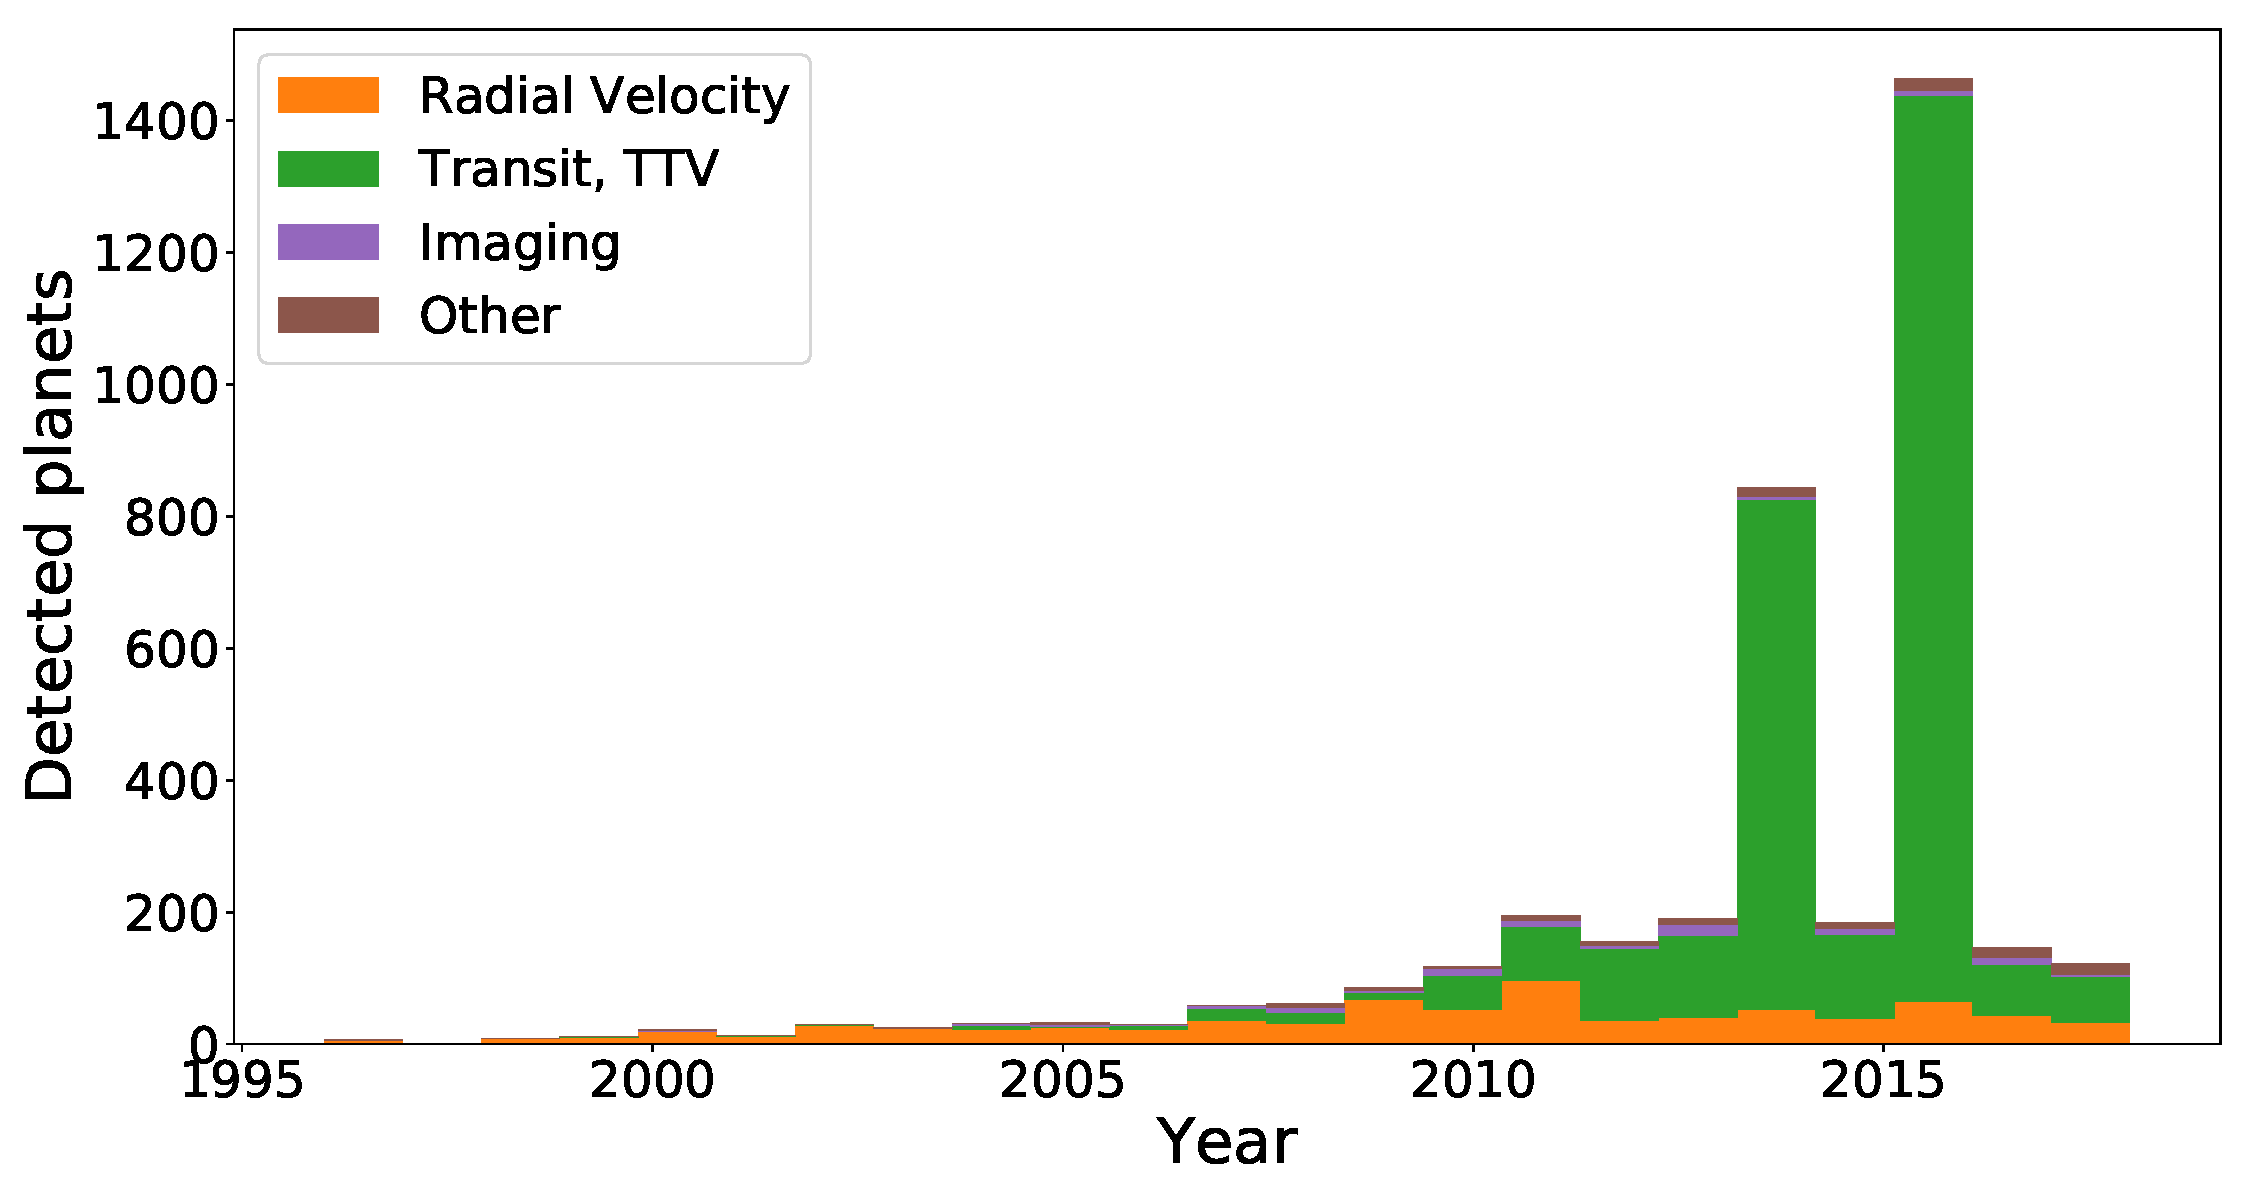
\includegraphics[width=0.7\linewidth]{./figures/introduction/exoplanetEU_year_method.pdf}
    \caption{Number of exoplanet detections per year separated by method (data from \href{http://ww.exoplanet.eu}{exoplanet.eu} October 2018).}
    \label{fig:detection_year_method}
\end{figure}


Details about the various main detection methods are provided in the following sections.

\subsection{Radial Velocimetry}
This techniques measures the radial velocity (RV) of the star by analysing the relative Doppler shift of its spectral lines due to the gravitational interaction with a companion.
As the star and companion orbit around their common centre of mass the spectrum of the star oscillates due to the change in relative motion to the observer as depicted in \fref{fig:rvdiagram-mayor}.
The key exoplanet property determined by the RV technique is the companions mass, or \mtwosini.
Where $i$ is the relative inclination of the orbital plane to the light of sight.

This method detected the first exoplanet around a solar-type star {51 Pegasi}~\citep{mayor_jupitermass_1995}, kick-starting the exoplanet field.
However, since the RV signal it arises from the gravitational interaction the RV method is more sensitive to large mass planet, on close-in orbits.
As such the first discoveries (\msini=0.47\Mjup{} orbiting at 0.05\AU{} for {51 Pegasi}) were surprising, unlike anything in our Solar System.
Several exoplanet discoveries followed in quick successions~\citep[e.g.][]{butler_planet_1996, marcy_planetary_1996} with many confirming the existence of the type of planets now referred to as ``hot-Jupiters''~\citep{butler_three_1997, charbonneau_detection_2000}.

The radial velocity amplitude of the first exoplanets detected were XXX \kmps....
The radial velocity signal of the Earth in a 1 year orbit around a solar-type star however is 8.9\cmps{}\citep{figueira_radial_2010}.
Specially constructed spectrographs, such as HARPS~\citep{mayor_setting_2003)} along with improve reduction techniques~\citet{lovis_new_2007} spectrographs in the optical pushed this mass detection limit down to the \mps{} level.\textbf{ Figure XX shows the mass of detected exoplanets over time decrease} \todo{Mass verse time plot}.
ESPRESSO~\citep{pepe_espresso_2014, megevand_espresso_2014} is the next generation high precision optical spectrograph aiming to push the detection limits to 10\cmps, to detect an Earth twin.

Most RV detection has been performed using optical spectrographs. However, as the amplitude of RV signal is inversely proportional to the mass of the star (RV $\propto M_{\star}^{-2/3}$), there is some focus on smaller mass M-dwarf stars. M-dwarfs are inherently cooler and thus emit a majority of their stellar output in the near-infrared {cite an M-dwarf paper?}, requiring dedicated \nir spectrographs such as {CARMENES}, {NIRPS}, and {SPIRou}.

\begin{figure}
    \centering
        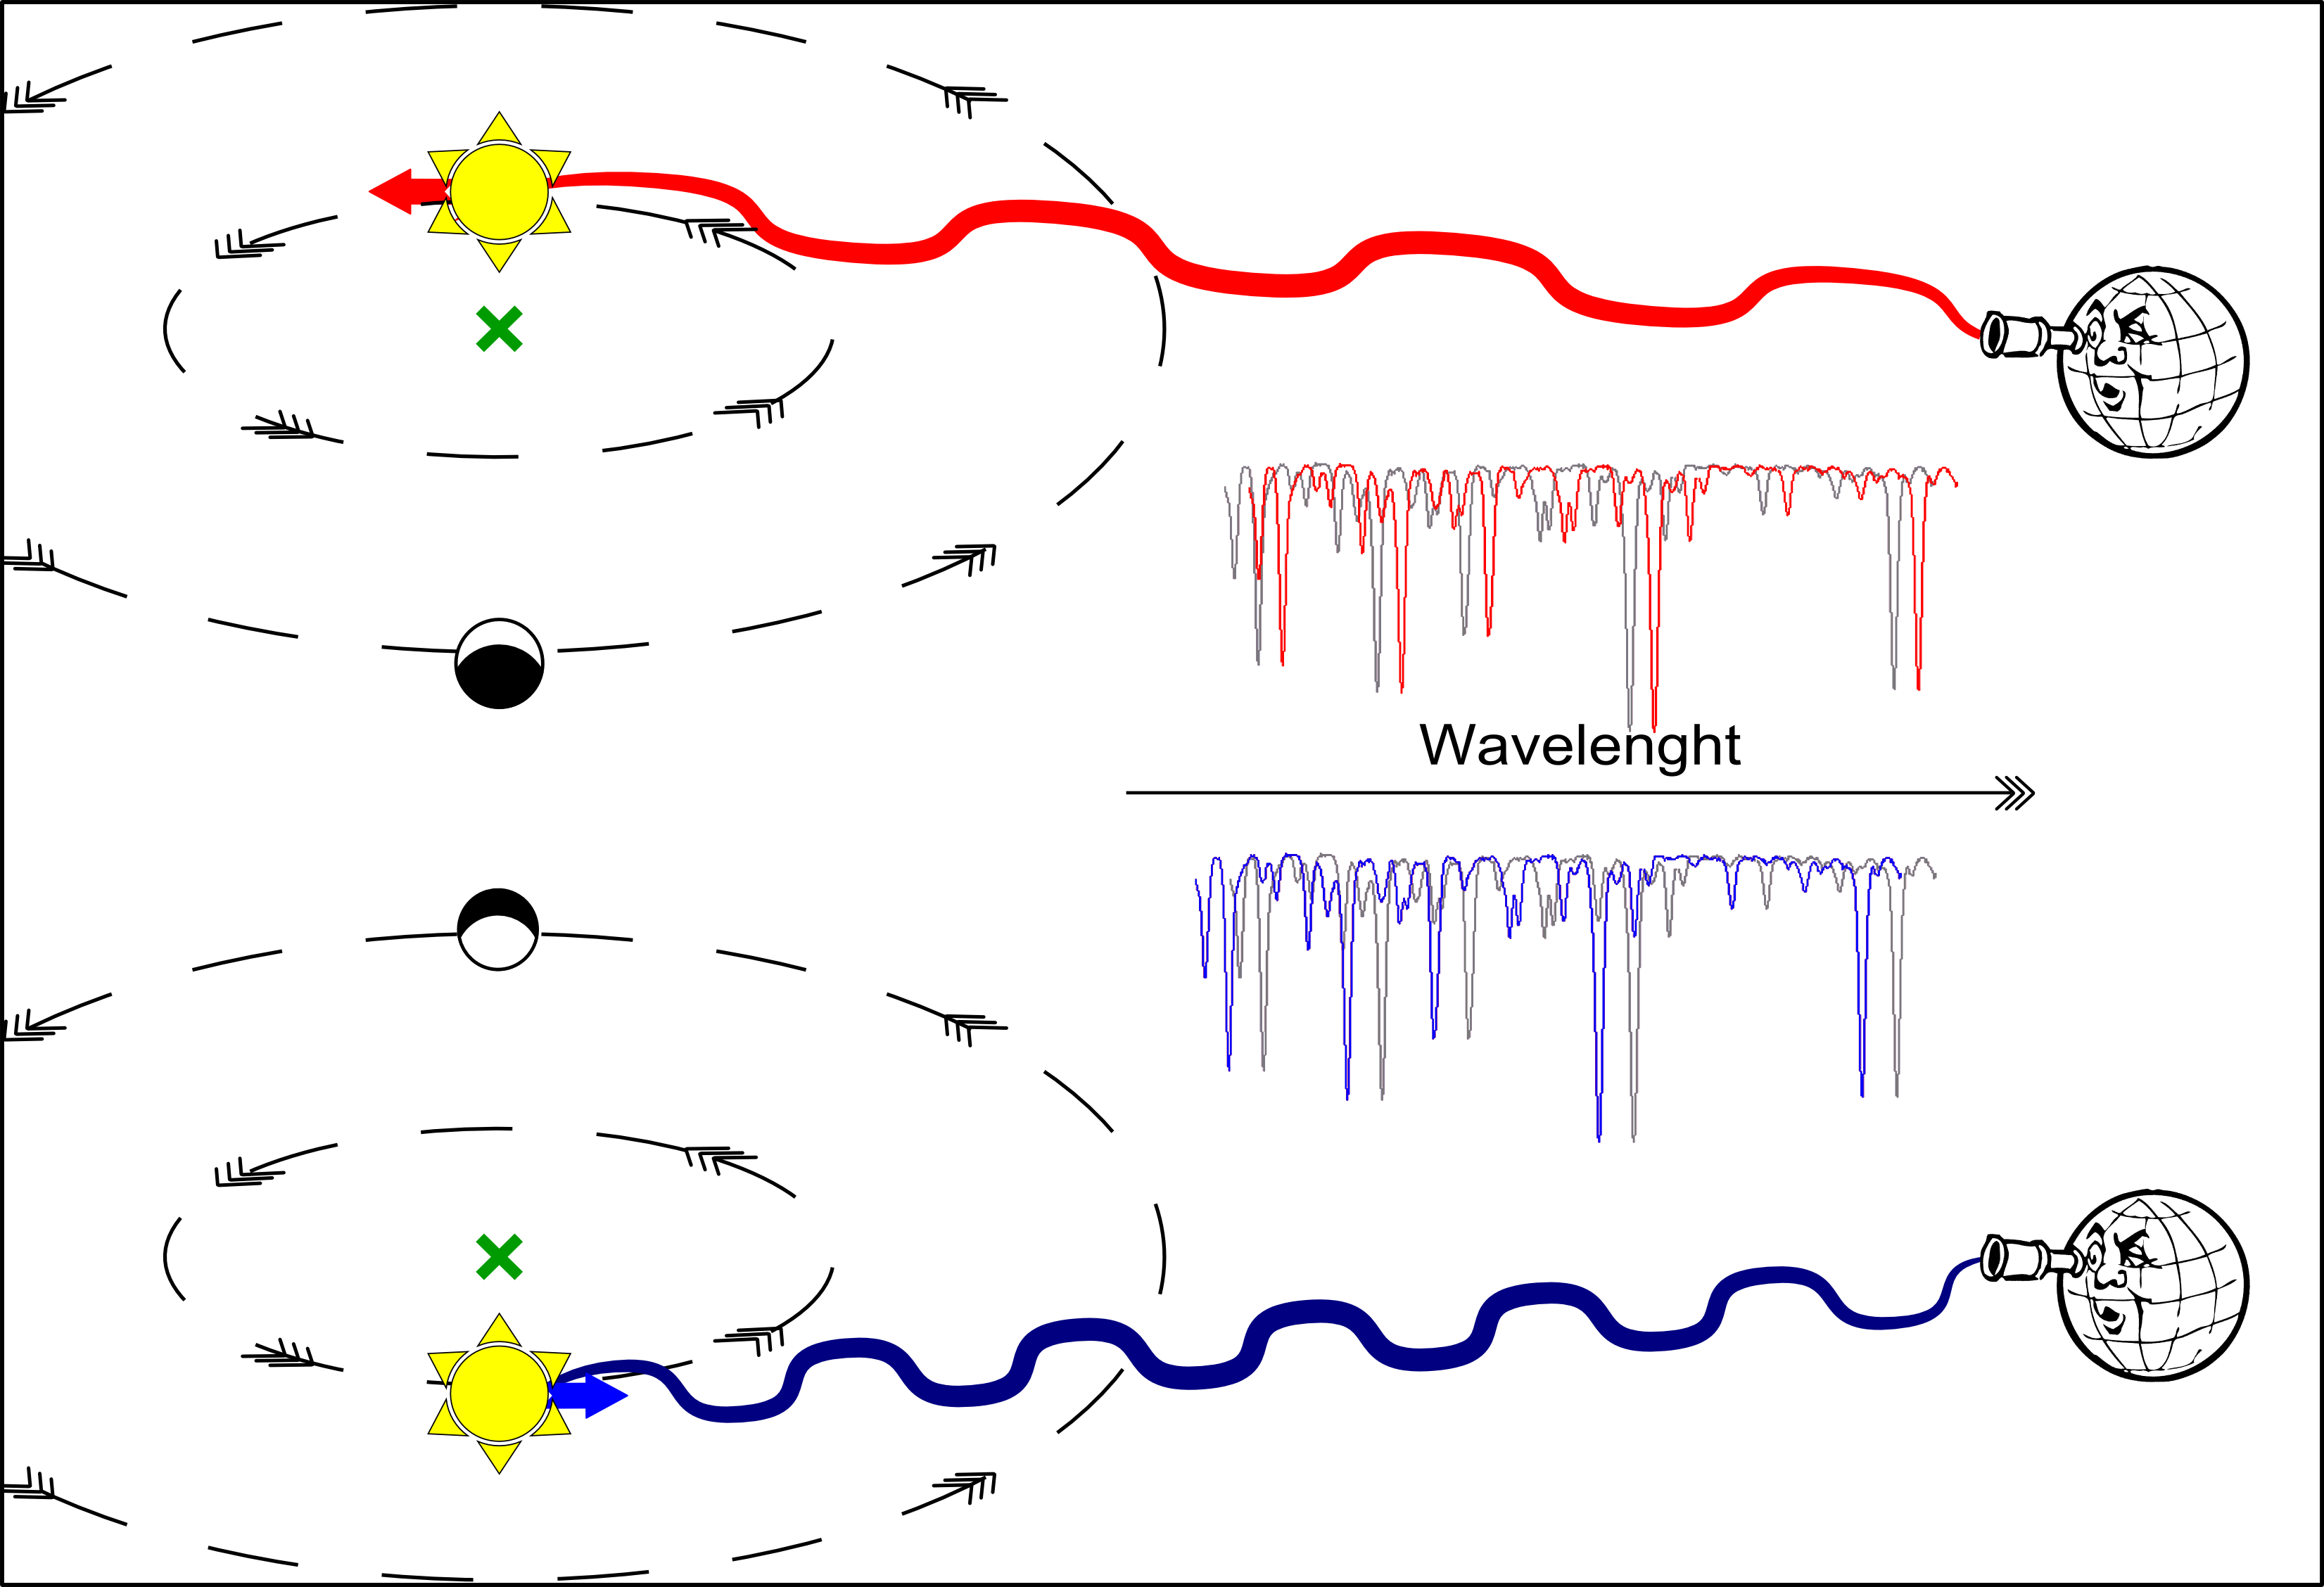
\includegraphics[width=0.45\linewidth]{./figures/introduction/RV_Diagram}
    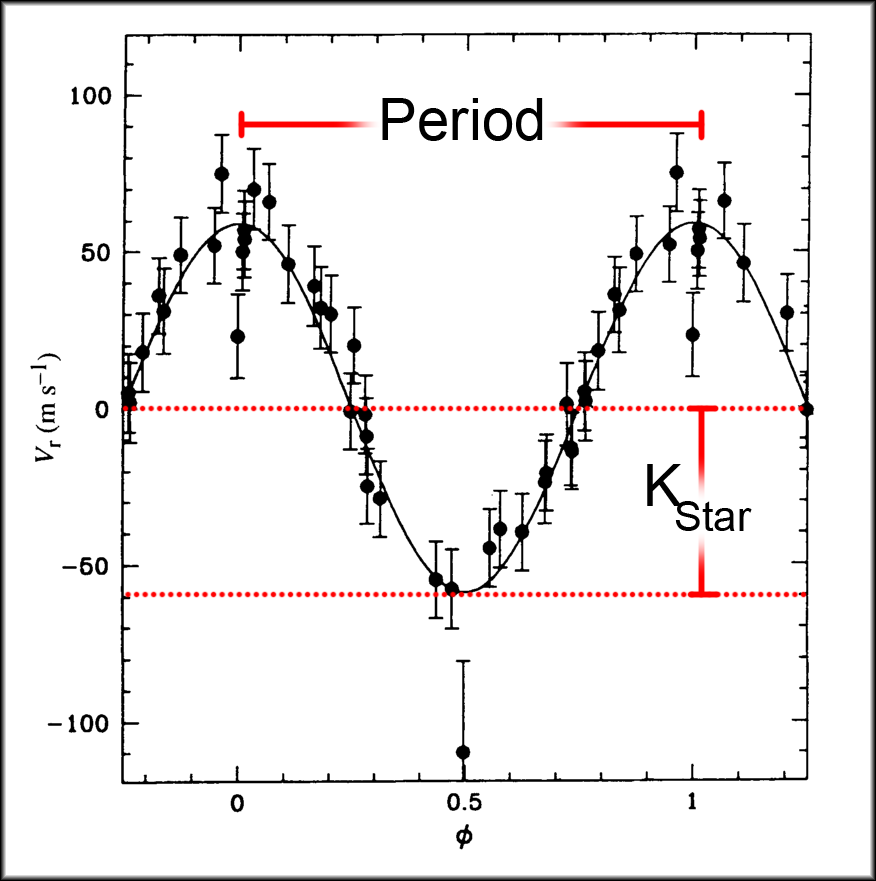
\includegraphics[width=0.3\linewidth]{./figures/introduction/PhaseFolded_51Pegb_Mayor_et_al_1995}
    \caption{Left: Diagram of {RV} method. Right: {RV} variation for the detection of {51 Pegasi}. Credit:~\citet{mayor_jupitermass_1995}}.
    \label{fig:rvdiagram-mayor}
\end{figure}


activity induced signals, rotation period?

\subsection{Transit methods}
The transit method detects the presence of a exoplanet by observing the periodic dimming of the star due to the passage of the exoplanet between the star and observer, partially blocking the star.
Geometry requires the orbit of the exoplanet needs to be aligned edge-on to the light of sight (low inclinations) for a transit to occur.
The geometric probability, $P$, that a exoplanet transits is estimated by 

\begin{equation}
P \approx \frac{R_{\star}}{a(1-e^^2)},
\end{equation}

where \(e\) is the eccentricity of the orbit, $R_{\star}$ is the star radii and \(a\) is the semi-major axis of the orbit (star-planet distance)~\citep{barnes_effects_2007}.
The probability increase with the size of the star but decreases with distance to the star.

The drop in stellar brightness during the transit allows the measurement of the planet/star radius ratio:
\begin{equation}
    \frac{\Delta L}{L} \sim \left(\frac{R_p}{R_{\star}})\right)^2
\end{equation}
where \(L\) is the luminosity of the star, \(\Delta L\) is the maximum luminosity variation (transit depth), and \(R_{\star}\) and \(R_p\) are the radius of the star and planet respectively.
\missingfigure{transit shape}


There are several other astrophysical phenomena which can mimic transiting exoplanet signals, created by configurations of two or more stars which may not involve an exoplanet. 
For example a transiting low-mass or white-dwarf star, grazing binary stars, or a transit in a multi-star system~\citep[e.g.][]{Cameron 2012, Santerne 2013}.
Follow-up RV observations (e.g Santerne 2011) are usually required to confirm the planets existence. 
Statistical validation techniques are also possible, such as the PASTIS software~\cite{diaz_pastis_2014}, when follow-up can not be performed.
With RV follow-up~\citet{santerne_sophie_2012} found a false positive rate as high as 35\% for short period giant planets, while~\citet{santerne_2016} found a 54.6\% false positive rate of 129 giant planet with periods less than 400 days. These sub-sample false positive rates are however higher than the global false positive rate of 9.4\%~\citep{Fressin_false_2013}/ 11.3\%~\citep{santerne_contribution_2013} found for Kepler.
Some of the currently known exoplanet systems with the smallest radii and lightest mass have been detected through transit and confirmed with high-precision RV follow-up~\citep[e.g.][]{queloz_corot7_2009, pepe_earthsized_2013, lopez-morales_kepler21b_2016, ment_second_2018}

The transit of a single planet can not directly determine the planetary mass.
However in multiple planet systems, the masses and sometimes the presence of other planets in the system can be determined from perturbations in the transit time and duration~\citep[e.g.][]{holman_use_2005, holman_kepler9_2010}.
A large number of systems have been detected that show transit timing variations (TTV) and transit duration variations (TDV) \citep[e.g.][]{holczer_transit_2016}.
The statistical validity of multi-transiting planets is also higher than single planets as probability of multiple false positive is lower than having multiple planets in the system~\citet{lissauer_almost_2012}.

The presence of star spots on the surface of a star can be observed in transit.
A star spot is a dark region on the stellar surface due to magnetic fields, which decrease the luminosity slightly.
If an exoplanet passes in front of a spot, the luminosity decrease from the spot is temporarily hidden and a small bump occurs in the transit shape.
The presence of spots in successive transits can indicate the alignment of the stellar rotation to the planet orbital plane~\citet{Sanchis-Ojeda et al 2012}.
An image from the 2012 transit of Venus in shows several dark Sun spots along sided Venus in \fref{fig:transit_venus} (although Venus did not cross them).
In this instance, unlike for other stars, the Sunspots can be spatially resolved.

\begin{figure}
    \centering
    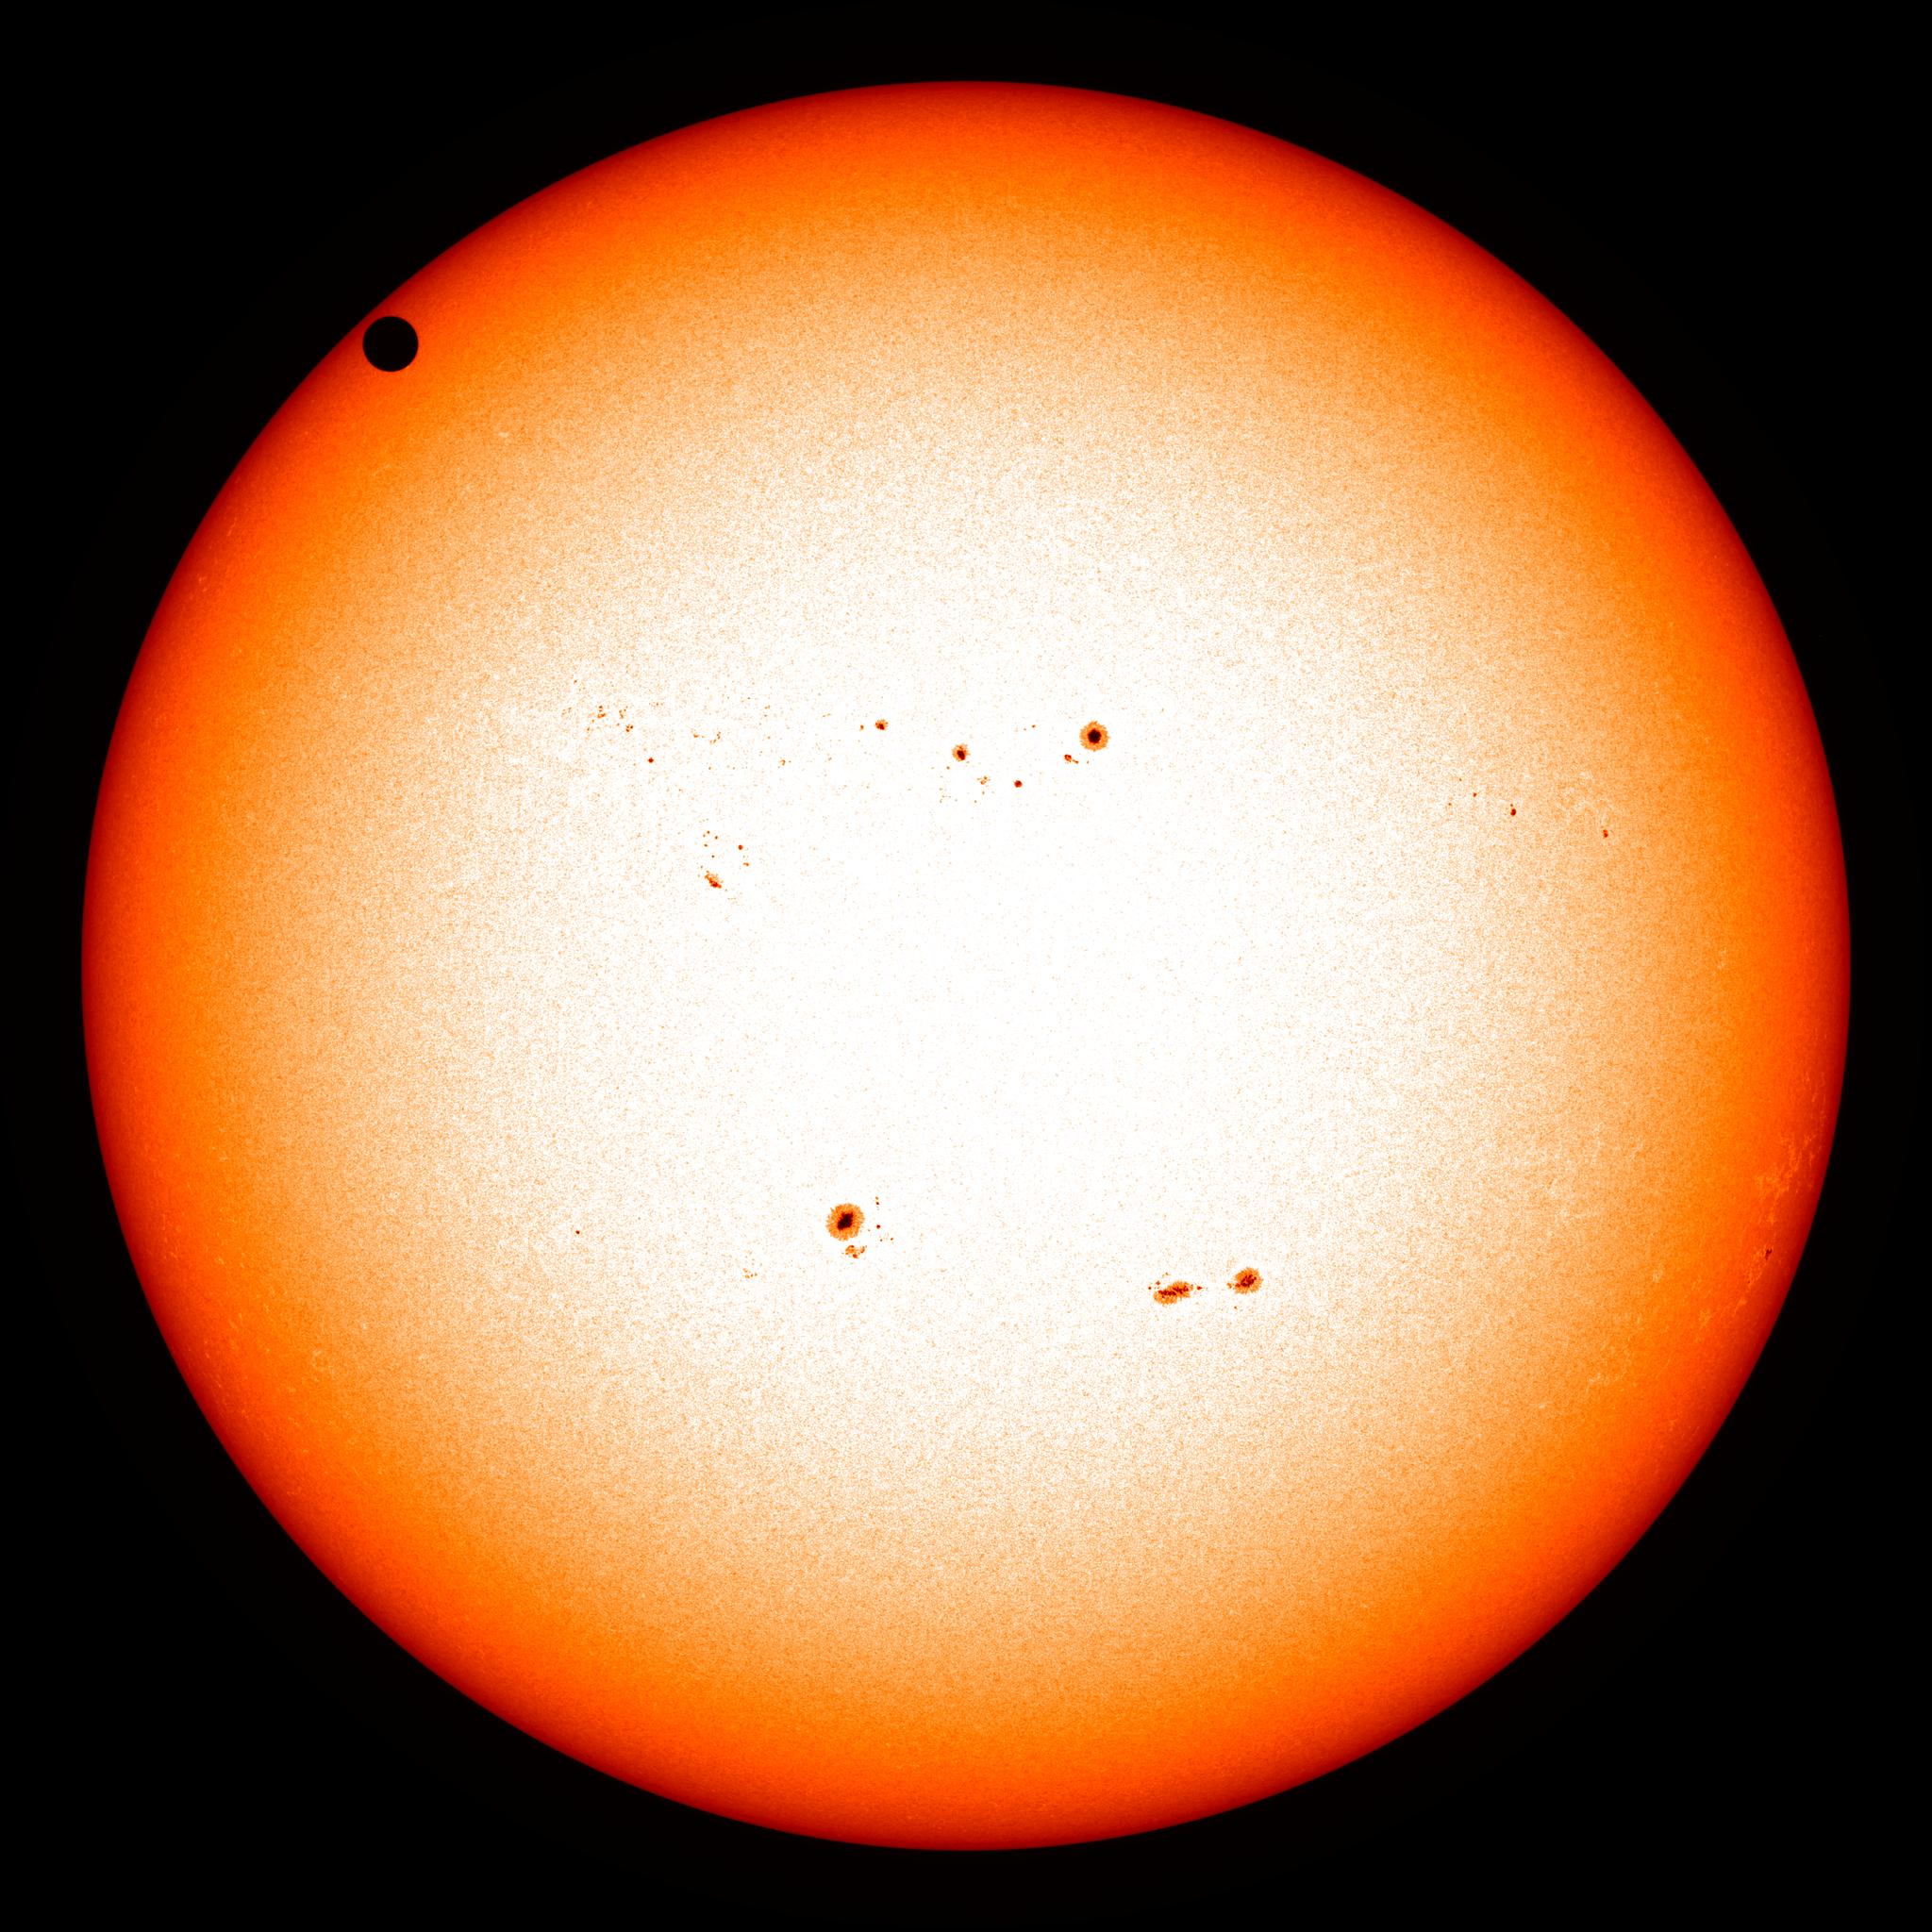
\includegraphics[width=0.3\linewidth]{./figures/introduction/SDO_2012_Venus_Transit.jpg}
    \caption{The 2012 transit of Venus obtained from Solar Dynamics Observatory satellite. Venus is the dark circle in the top left of the Sun. Limb darkening is observed as the change in colour/brightness from white to red near the edge. Several sunspots are also observed on the surface of the Sun. Credit: NASA/SDO, HMI}
    \label{fig:transit_venus}
\end{figure}


The vast majority of transit detections have come from Kepler\citep{borucki_characteristics_2011}, which focused on a small patch of sky (0.25\%) for four years continuously.
However, {CoRoT} \textbf{(barge 2008)} and ground-based surveys are also WASP~\citet{pollacco_wasp_2006}, OGLE~\citep{udalski_optical_2002}, TreS~\citep{alonso_tres1_2004} have also had successful transit detections.

Following in the footsteps of Kepler the next generation transit hunter TESS~\citep{ricker_transiting_2014} has already announced discoveries of new transiting planets only months after launch \citet{vanderspek_tess_2018, gandolfi_tesss_2018, huang_tess_2018}.
It will eventually cover more than 90\% of the sky with impressive planetary yield expected of ~10000 exoplanets, with around 3500 the size of Neptune or smaller~\citep{barclay_revisded_2018, huang_expected_2018}.
However, the observation coverage is not uniform, with the majority of the ecliptic plane receiving only one month of observations, limiting the detection sensitivity to short period transiting planets.


\subsection{Direct detection}
\
\subsection{Astrometry}

Measuring the motion of the stars in the sky

Previously with Hipparcos.
The most precise parallax measurements are being perform with GAIA, with...


\subsection{Microlenseing}


Notable discoveries section? Proxima b?  


\subsection{planet validation}
After the few mehtods tlakj abnuot the issuesfollowup confirmation

Activity indiuced RV
Mimiking signals false postives

PASTIS Diaz



\subsection{Detecting atmospheres}

\subsection{Transmission spectroscopy}

\subsection{Reflection in optical}

Transit and occulations~\citet{winn_transits_2010}


\begin{figure}
    \centering
    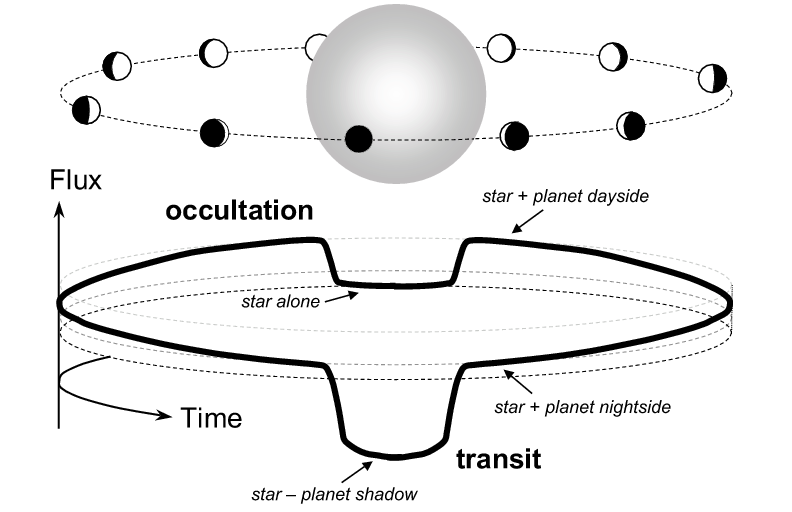
\includegraphics[width=0.6\linewidth]{./figures/introduction/circular_diagram.png}
    \caption{Illustration of transits and occultations. Only the combined flux of the star and planet is observed. During a transit, the flux
        drops because the planet blocks a fraction of the starlight. Then the flux rises as the planet’s dayside comes into view. The flux drops
        again when the planet is occulted by the star.~\citet{winn_transits_2010}}
    \label{fig:transits_and_occultations}
\end{figure}
\todo{caption directly from source- maybe adapt??}

\subsection{Phase variations}

\subsection{High resolution spectroscopy}
Snellen  Brogi, de Kok

Cross correlation mle  Piskorz 2016


\subsection{Stellar and planetary formation}

Brown dwarfs

\subsection{Exoplanet distribution} 4 different groups

\fref{}


\begin{figure}
    \centering
    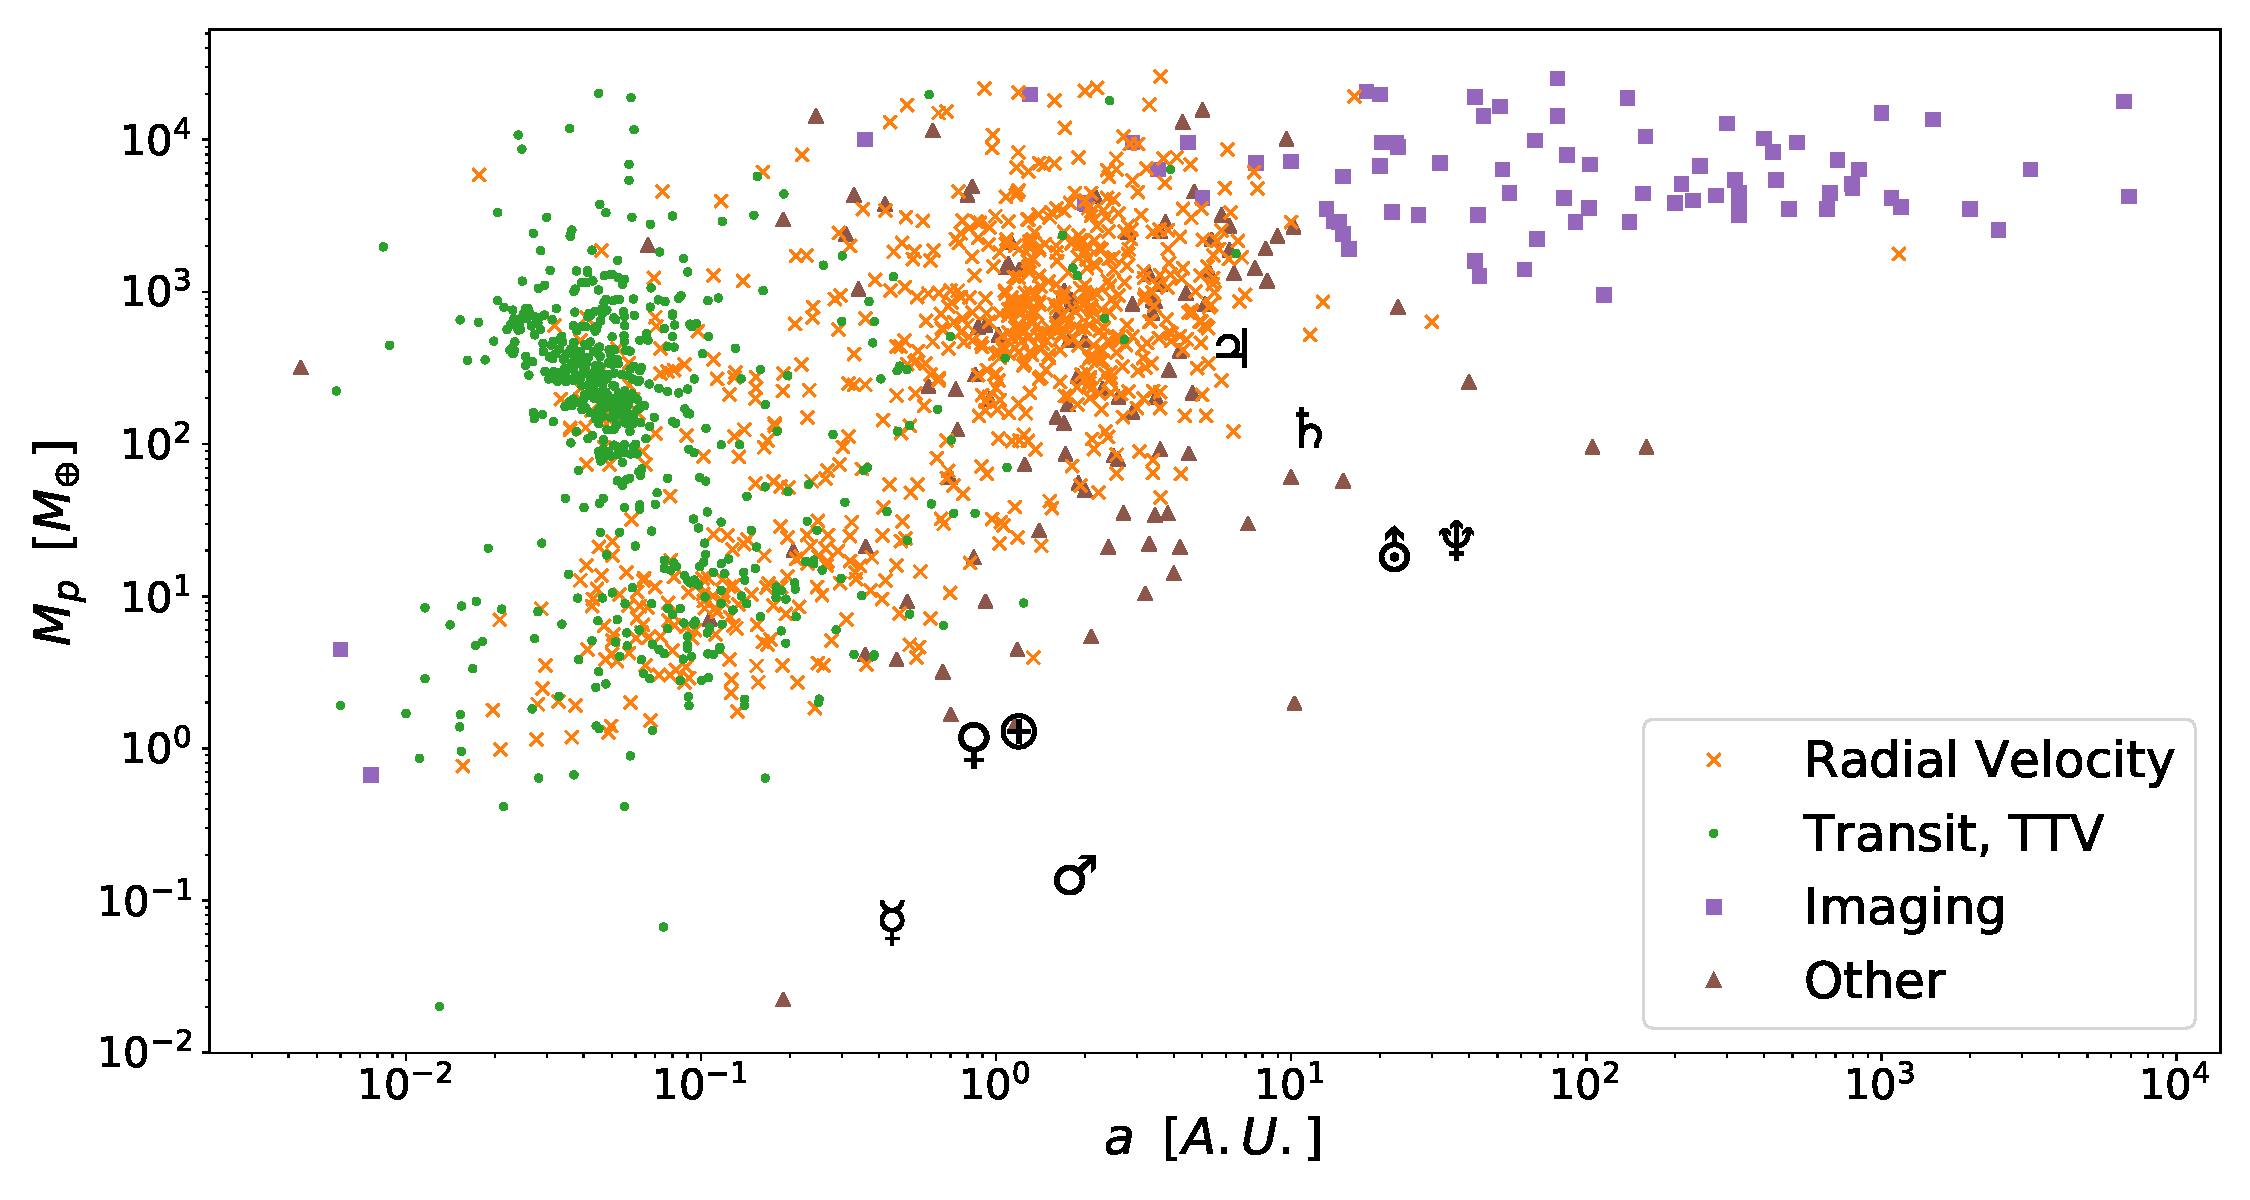
\includegraphics[width=0.7\linewidth]{./figures/introduction/exoplanetEU_a_mass.pdf}
    \caption{Distance mass diagram (data from \href{http://ww.exoplanet.eu}{exoplanet.eu} October 2018)}
    \label{fig:pltoverlayadd}
\end{figure}


Explore what these method have found with exoplanet populations.

The discovery of the hot-Jupiter class (large mass planets on close in orbits) challenged the accepted planet formation theories at the time~\citep[.e.g][]{pollack_formation_1996}(jorge thesis) in which our Solar System was thought to be typical with small rocky planets close to the Sun and large giant planets further away.


super earth wolf503b - recent detection


MR relation ship image arXiv:1506.05097~\citet{chen_probabilistic_2016}

\begin{figure}
    \centering
    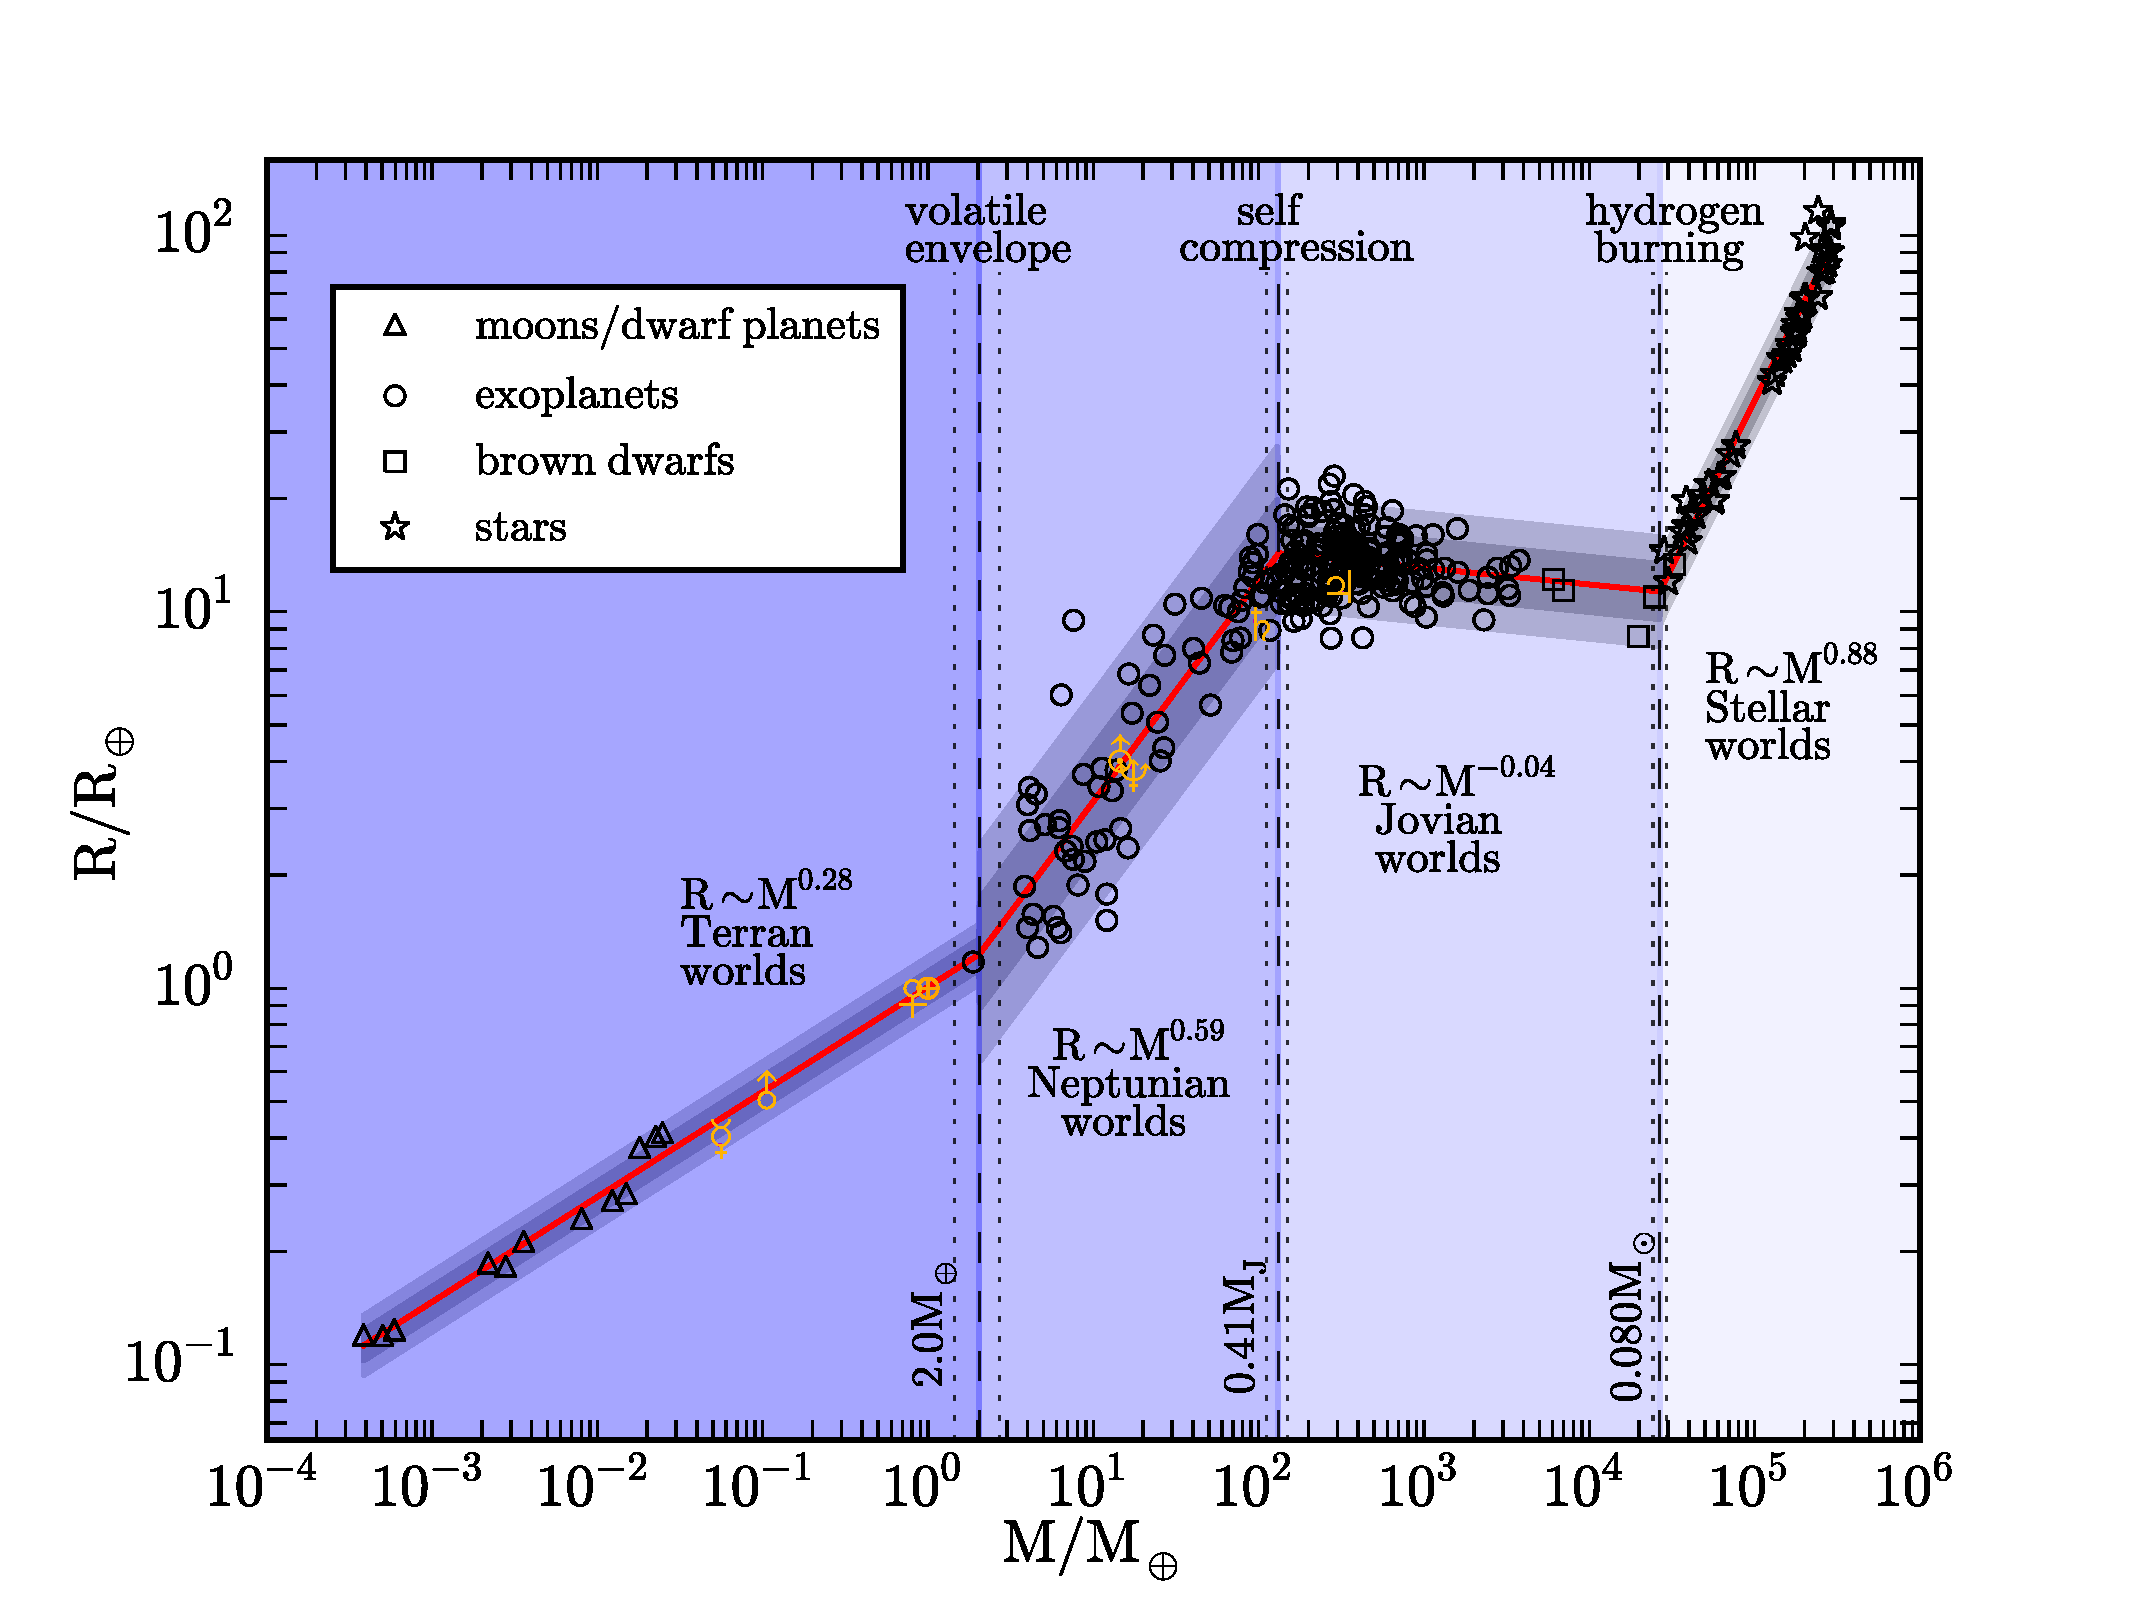
\includegraphics[width=0.4\linewidth]{./figures/introduction/mass_radius_relation.pdf}
    \caption{M-R relationship~\citet{chen_probabilistic_2016}}
    \label{fig:mass_radius_relation}
\end{figure}

Santos et al 2017 \todo{read and quote}


double peak histogram from an rv paper?? Faria 2018?


did they form from the molecular cloud when the star was forming or from the reminantes of the disk after the star formed like exoplanets....?


\section{ conditions for life?}
habitable zone stuff
proxima b
Jorges paragraph.... 

\section{Main Section 2}


Spectral Disentangling techniques
- PSOAP
- Differencing Fruluga
- Templates?


2D-cross-correlation?   Piskorz 2016 seems to have promising technique


\section{Recent detections in Companion spectra.}

Birkby


\subsection{model fitting transit stars (not actual title, more other similar methods)}
There are other situations in which to determine the presence of faint secondary spectra, such as, identifying the presence of any background or companion stars of transiting planet candidates. Many astronomical phenomena such as grazing eclipsing, a giant primary star eclipsed by a dwarf or a background star can produce signals indistinguishable from planetary transits. Efforts to characterize the false positive probability (FPP) among Kepler planet candidates is as high as $\sim35\%$~\citep{santerne_sophie_2012}. The presence of unknown companions or background stars decreases the dimming effect from the planet transit leading to smaller planetary radius. Where multiple stars are present there may also be ambiguity on which star hosts the planet.~\citet{kolbl_detection_2015} developed a method for detecting the presences of faint secondary lines in optical stellar spectra by matching observations to the SpecMatch library of stellar spectra. Identifying the spectroscopic evidence of a secondary star for 63/1\,160 California \emph{Kepler} Survey objects of Interest (KOI).


For transiting planets that presence of a background star or a companion star causes problems in characterizing the planet. Being able to detect spectra signal of the a faint second spectra in double-lined spectroscopic binaries.
For example eclipsing binaries,
A dim binary system companion or a giant planet around a background star can mimic the transit of a small Earth-like planet on a foreground star.






\subsection{Earths atmosphere}
While the Earth's atmosphere is important for an Astronomer's lungs, it can be a nuance for their ground-based observations. As light form astronomical sources passes through the atmosphere, its molecular components absorb some of the light, changing spectral components observed by imprinting a transmission spectrum of our atmosphere. The \ce{H2O} absorption is a key example as it defines the photometric and spectroscopic bands in the \nir{}. \missingfigure{example to point to}.

The correction of observations from the contamination of Earth's atmosphere is a complex process. The transmission is variable on many different time scales, the water vapour change is rapid, concentrations of atmospheric constituents, to seasonal and longer. Such as the increase in atmospheric \ce{CO2} causing anthropamorphic climate change this requires 6\% change to \ce{CO2} line depths since 2000 Molecfit paper? There is also variation with airmass, which depends on the observation angle in the sky and changes as targets move across the sky during the night.

other constituents, \ce{CO}, \ce{CO2}, \ce{CH4} \ldots{}, angle of observations.

An important consideration in the detecting the constituents of planetary atmospheres is the characterization and removal of Earths telluric lines.

e.g.\ 50\% error in \ce{CO2} detection on Mars atmosphere


Recently~\citet{ulmer-moll_telluric_2018} compared the telluric correction possible from three different synthetic telluric software against the standard star model. Molecfit, a software from ESO was the most.

This is a growing field and there are other software available too\ldots{}


Water vapour content has rapid variability. Works such as Snellen 2011, \ldots{} \ldots{}  model the telluric variation during a observations to remove telluric lines and detect planetary lines.

\todo{finish this}


Telluric absorption map
\begin{figure}
    \centering
    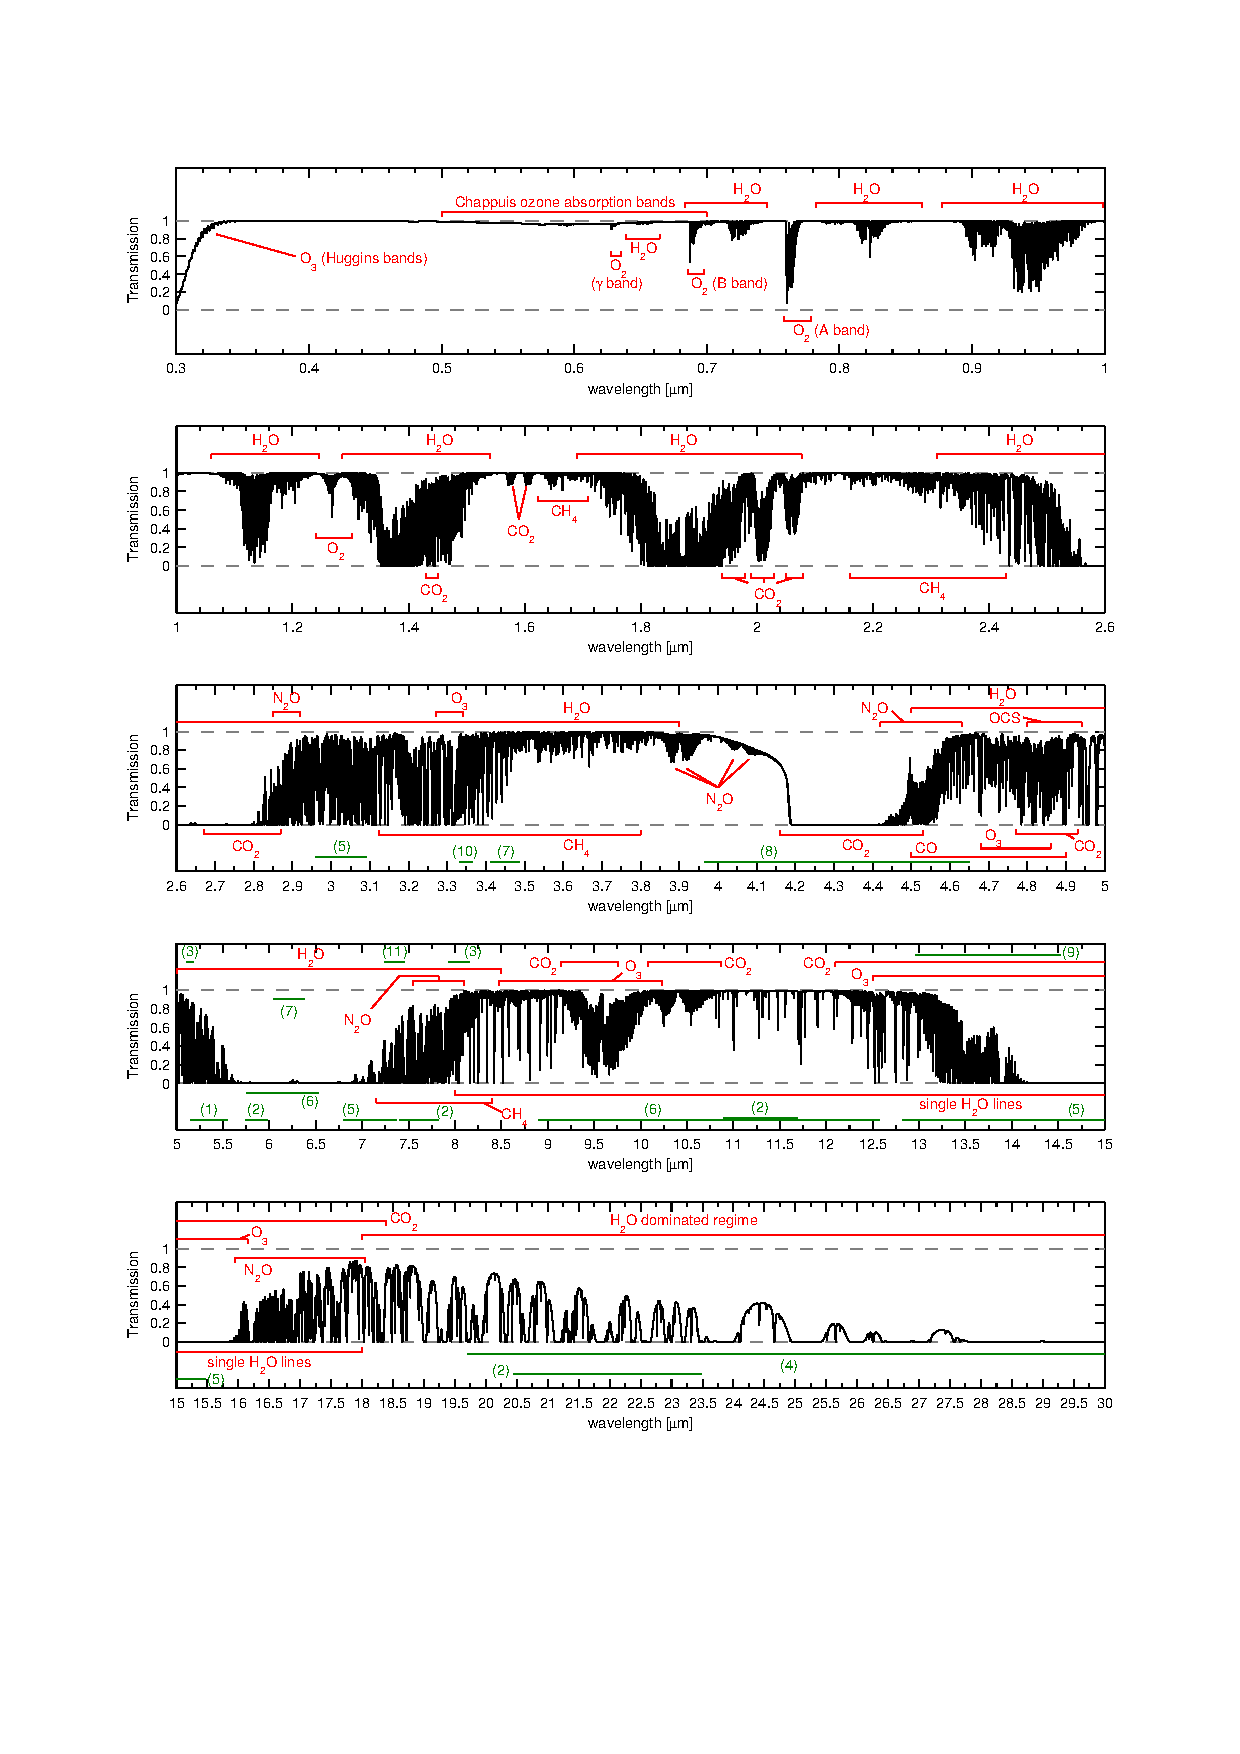
\includegraphics[width=0.9\linewidth]{figures/advanced_material/cropped_molecfit_absorbtion}
    \caption{Reproduction of Figure~1 of~\citet{smette_molecfit_2015} showing telluric absorption form 0.30 \um. Original caption:}
    \label{fig:croppedmolecfitabsorbtion}
\end{figure}
\todo{Add original caption to \ref{fig:croppedmolecfitabsorbtion}}




\section{Paper Introduction}
\label{sec:intro}
Brown dwarfs (BDs) are sub-stellar objects unable to achieve hydrogen fusion, with masses around \(13-80~\textrm{M}_{jup} \)~\citep{chabrier_theory_2000}, bridging the gap between low-mass stars and giant planets. Without sustained fusion, brown-dwarfs cool down over time with an age-dependent cooling rate. Therefore, there is an inherent degeneracy between the mass, age and luminosity of a given BD\citep{burrows_nongray_1997}. This degeneracy may be broken by observation of several parameters, for instance when a BD is in a binary system with a main sequence host star, using both the host stars age and the masses derived from the dynamical motion.

A paucity of BD companions exists in short period orbits around Sun-like stars (\(\lesssim5 \)\,AU), compared to stellar or planetary companions, termed the \emph{brown dwarf desert}~\citep{halbwachs_exploring_2000,zucker_analysis_2001,sahlmann_search_2011}. As the number of known BDs orbiting solar type stars is low, the characterization of benchmark BDs in the brown dwarf desert~\citep[e.g.][]{crepp_trends_2016} is beneficial in understanding this sub-stellar population and to help constrain formation and evolution theories~\citep{whitworth_formation_2007}. The BD desert also provides a greater challenge as it reduces the amount of good BD candidates to study.

BDs in binary systems, unlike free-floating BDs, allow for the determination of their masses, when complemented with radial velocity ({RV}) and astrometry measurements. The {RV} technique provides the mass lower-limit (\mtwosini{}) of binary and planetary companions, while complementary astrometry measurements can often provide mass upper-limits~\citep[e.g.][]{sahlmann_search_2011}. Measuring or tightening the constraints of BD masses improves the understanding of mass dependence on BD formation processes. For instance, there is growing evidence that the larger giant planets and BD companions do not follow the well known metallicity-giant planet correlation seen in main-sequence stars with planets~\citep[e.g.][]{santos_spectroscopic_2004,santos_observational_2017, maldonado_searching_2017}. Photometry along with stellar evolution models~\citep[e.g.][]{baraffe_evolutionary_2003,allard_btsettl_2013} can also be used to estimate the mass of BD companions~\citep[e.g.][]{moutou_eccentricity_2017} if there is sufficient orbital separation, and a precise determination of the age~\citep{soderblom_ages_2010}.

Recently, there has been a renewed interest in BD candidates triggered by exoplanetary searches. While several works found similar properties on the two populations, like a similar density~\citep{hatzes_definition_2015}, others found intriguing differences. One of the most recent is the different host metallicity of the Brown Dwarf and giant planet populations~\citep{santos_observational_2017, schlaufman_evidence_2018}, a very strong hint of different formation mechanisms.

Spectral observations of binary systems contain the spectra of both bodies, in proportion to their flux ratio, and Doppler shifted relative to each other due to their orbital motion. One technique to recover the spectra of the companion is secondary reconstruction through a differential spectrum~\citep{ferluga_separating_1997}. Spectra from different phases are shifted to the host stars rest frame and subtracted to mutually cancel out the spectrum of the host star allowing the faint companion spectra to become visible. Advances in high-resolution and near-infrared (\nir{}) capabilities should enable this technique to be applied to BDs and planet companions, in which smaller {RV} shifts can be resolved and the contrast ratio of the smaller companion is improved.

Observing in the \nir{}is specifically desirable for the cooler sub-stellar and giant planet companions as their thermal emission is stronger in the infrared compared to the optical. This improves the contrast ratio between the host star and companion, providing favourable conditions for their detection and spectral separation. CRIRES, a high resolution \nir{}spectrograph, has made many prominent advances in recent years with the detection of atmospheric constituents, such as \(\textrm{CO} \) and \(\textrm{H}_{2}\textrm{O} \), atmospheric winds and thermal profiles, rotation and orbital motion, for both transiting and non-transiting planets~\citep[e.g.][]{snellen_orbital_2010, brogi_signature_2012, rodler_weighing_2012, dekok_detection_2013, brogi_carbon_2014, snellen_fast_2014, piskorz_evidence_2016, brogi_rotation_2016, birkby_discovery_2017}.

The higher temperature and relatively larger size of BDs compared to giant-planets makes the development of spectral recovery techniques for BD companions a logical step towards the spectroscopic detection of planetary atmospheres. There has been the recent installation and continued development of many new high-resolution \nir{}spectrographs, such as, {CARMENES}~\citep{quirrenbach_carmenes_2014}, NIRPS~\citep{bouchy_nearinfrared_2017} or SPIRou~\citep{artigau_spirou_2014}, as well as, the CRIRES+~\citep{dorn_crires_2016} upgrade. These new instruments motivate the study of \nir{}-oriented methodologies for spectral recovery, and are of high importance due to the larger planet-to-star flux ratio provided by near-IR compared to the visible.

{\rd{} The search and detection of faint secondary spectra is not only relevant to planetary atmospheres.~\citet{kolbl_detection_2015} developed a method to detect the presence of optical secondary spectra down to a flux ratio of 1\% in the hosts of \emph{Kepler} transit candidates. The presence of which can cause ambiguities in the system configuration, and increase the uncertainty of the measured planet radius. The characterization of the false positive probability rate for Kepler has been found to be as high as  \(\sim\)35\%~\citet{santerne_sophie_2012}.}

In this paper we apply two different techniques on FGK stars with BD companions with the aim to spectroscopically detect their companions. In Sect.~ref{sec:data} we present the observations and reduction process as well as the spectral models used in this work. In Sect.~ref{sec:specdiff} we explain the differential spectral technique and its applicability to these observations while in Sect.~ref{sec:results} we apply companion recovery using a \textchisquared approach. In Sect.~ref{sec:discussion} we discuss our results and in Sect.~ref{sec:conclusions} we present our conclusions.



\section{Motivation}
